\chapter{Results} \label{ch:results}

\section{Introduction}
%introduce the results section and what processing will be done
The information gathered from the previous chapter is used to estimate the azimuth and elevation angles of the transmitter. First the azimuth angle will be estimated which will provide the information necessary for also calculating the elevation angle. The results of the estimation techniques are then analyzed to determine their accuracy.

%-----------------------------------------------------------------------------------------------------------------------------------------------------------------------

\section{Transmitter Azimuth Angle Estimation} \label{sec:transmitter_azimuth_angle_estimation}
%formulate the estimation equation and discuss ambiguity considerations
The azimuth angle estimation technique is based on the data collected by rotating the helicopter platform in a clockwise manner, during which a Doppler profile and subsequent maximum and minimum values are calculated. After a complete rotation the Doppler maximum and minimum values produce a sinusoidal pattern as shown in Figure \ref{fig:tx_azimuth_angle_200} without knowing the starting azimuth angle. With this data we find an unambiguous angle that will set the coordinate space and provide an estimate of current azimuth angle. To do this the absolute value of the minimum Doppler profile data is superimposed onto the maximum Doppler profile data as shown in Figure \ref{fig:azimuth_estimation_max_vs_absMin}.

\begin{figure}
	\begin{center}
		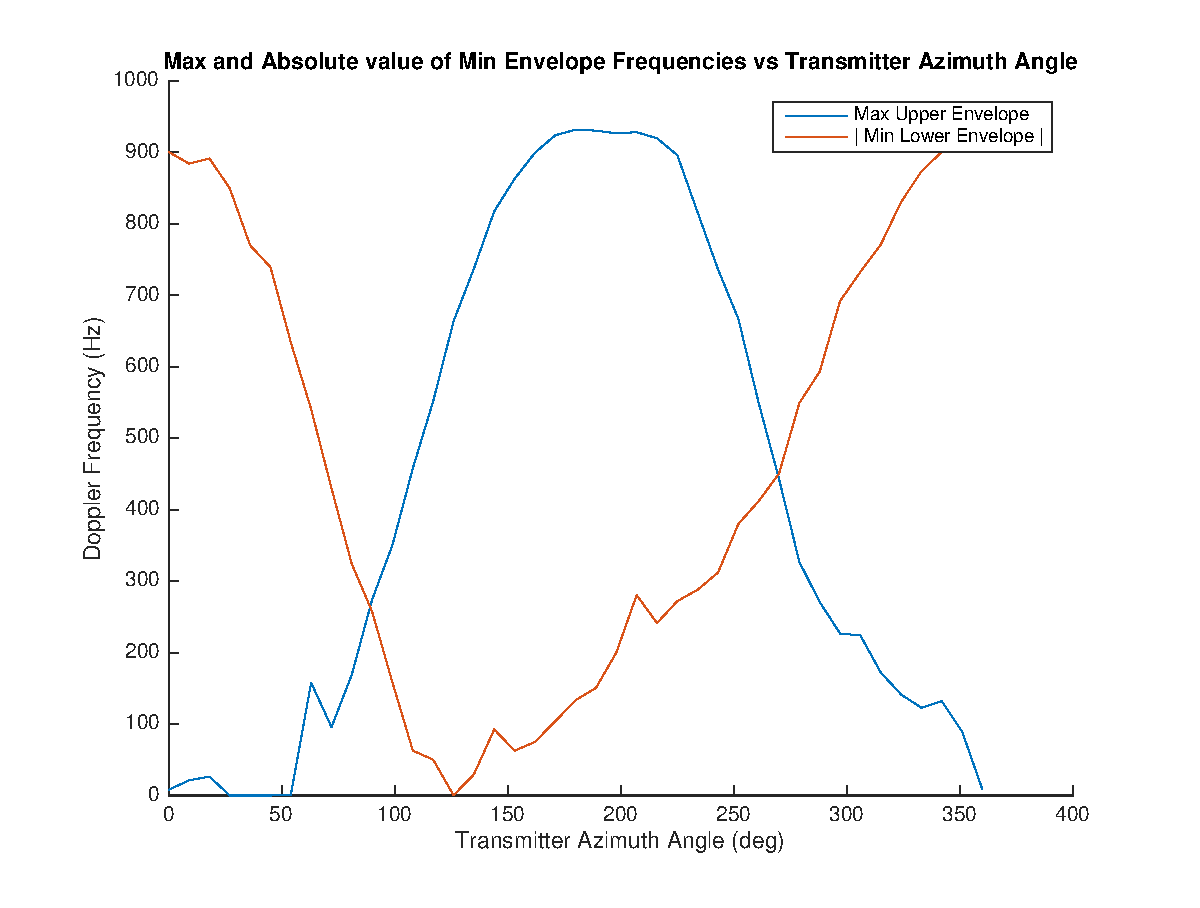
\includegraphics[width=10cm]{images/results/Azimuth_angle_estimation_max_vs_absMin.eps}
		\caption{Max and Absolute value of Min Doppler Profile Frequencies vs Transmitter Azimuth Angle at an Elevation Angle of 45\textdegree}
		\label{fig:azimuth_estimation_max_vs_absMin}
	\end{center}
\end{figure}

From Figure \ref{fig:azimuth_estimation_max_vs_absMin} there are two points at which the maximums and the absolute value of the minimums cross. We then take the difference:

%formula for difference
\begin{equation}
	 Profile Difference = Max Doppler Profile - | Min Doppler Profile |
	 \label{eqn:difference}
\end{equation}

where $Max Doppler Profile$ is an array of the maximum value of each upper profile calculation, and $Min Doppler Profile$ is an array of the minimum value of each lower profile calculation. The result is an almost exact sinusoid centered around zero, shown in Figure \ref{fig:azimuth_estimation_difference}.

 \begin{figure}[b]
	\begin{center}
		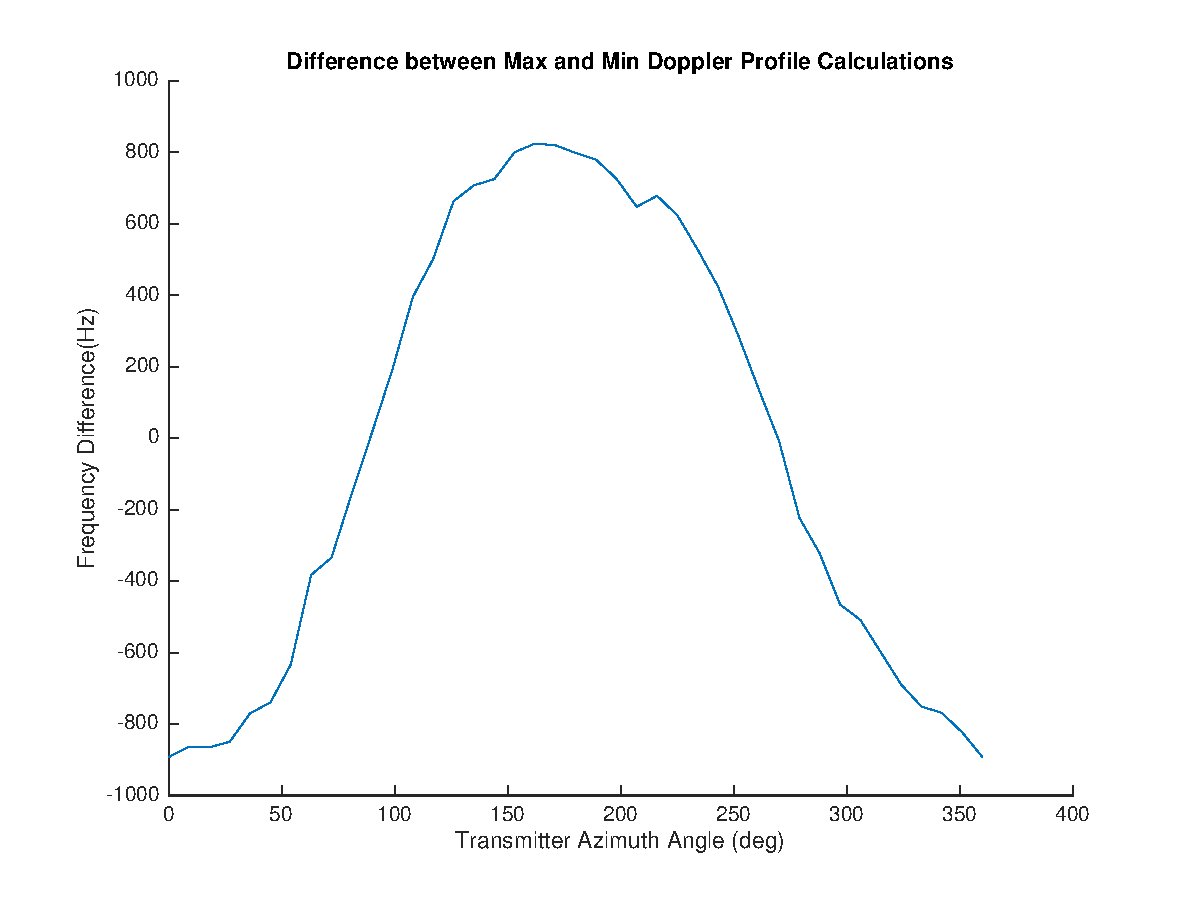
\includegraphics[width=10cm]{images/results/Azimuth_angle_estimation_difference.eps}
		\caption{Difference between Max and Min Doppler Profile Calculations vs Transmitter Azimuth Angle at an Elevation Angle of 45\textdegree}
		\label{fig:azimuth_estimation_difference}
	\end{center}
\end{figure}

While Figure \ref{fig:azimuth_estimation_difference} provides information about the angle of the transmitter it does not contain enough to locate an unambiguous azimuth angle in itself. Therefore by finding the correct Doppler for each azimuth, from the $Max Doppler Profile$ and the $| Min Doppler Profile |$, we can determine an unambiguous reference. This is done by evaluating the difference at each angle, and if the difference is negative the $| Min Doppler Profile |$ is used and if positive the $Max Doppler Profile$.

%matlab for corrected doppler
\begin{lstlisting}
%corrected Doppler frequency for processing
for i = 1:length(upper)
    if(difference(i) < 0)
       correct_fd(i) = abs(lower(i));
    else
       correct_fd(i) = upper(i);
    end
end
\end{lstlisting}

\begin{figure}
	\begin{center}
		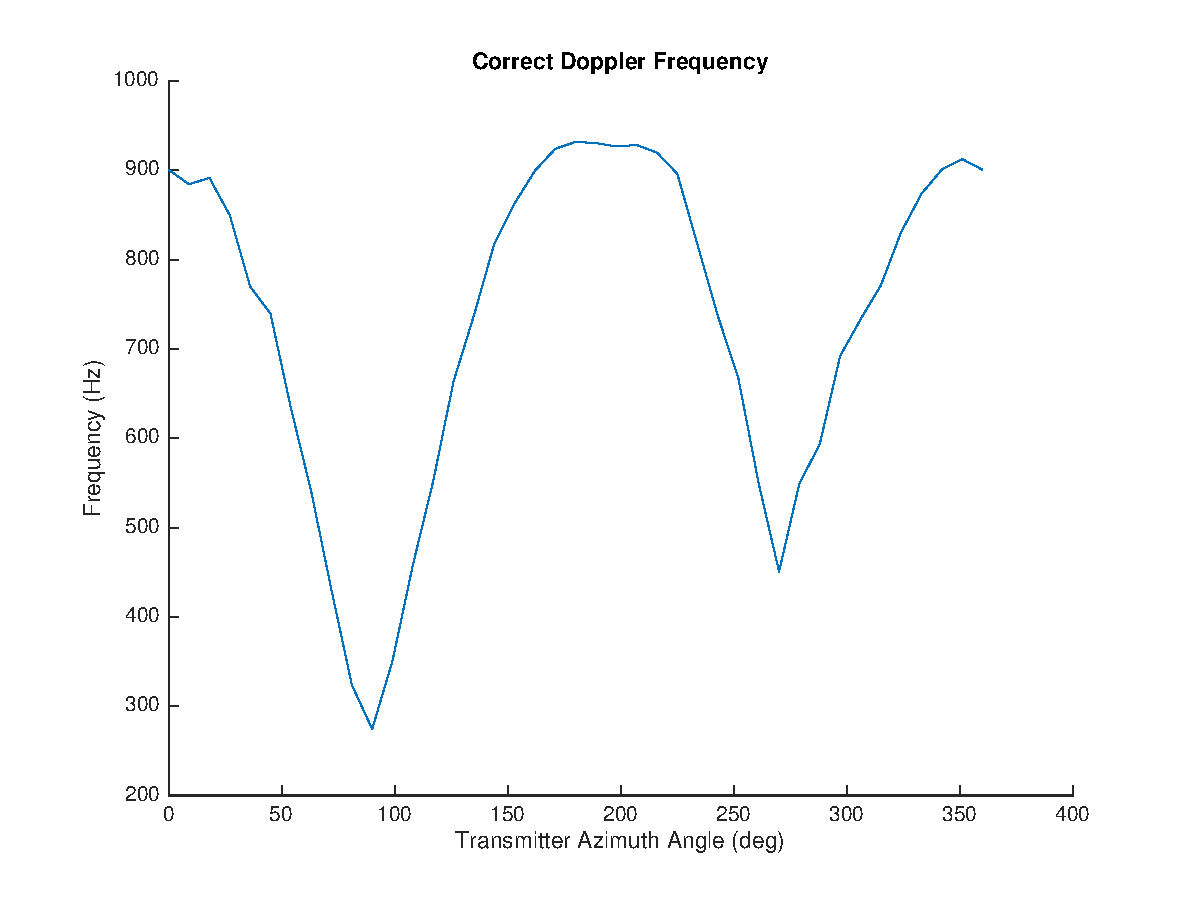
\includegraphics[width=10cm]{images/results/Correct_doppler.eps}
		\caption{Correct Doppler Frequencies vs Transmitter Azimuth Angle at an Elevation Angle of 45\textdegree}
		\label{fig:correct_fd}
	\end{center}
\end{figure}

The correct Doppler is shown in Figure \ref{fig:correct_fd} which displays the amount of Doppler that is currently acting on the signal for that specific azimuth angle. The data gathered contains a global minimum at 90\textdegree \space and a second local minimum at 270\textdegree. The 90\textdegree \space can be found easily by taking the minimum of the correct Doppler signal.

%matlab minimum code
\begin{lstlisting}
%Minimum of corrected Doppler
[Min,I_min] = min(correct_fd);
\end{lstlisting}

%figure of minimum located vs azimuth
\begin{figure}
	\begin{center}
		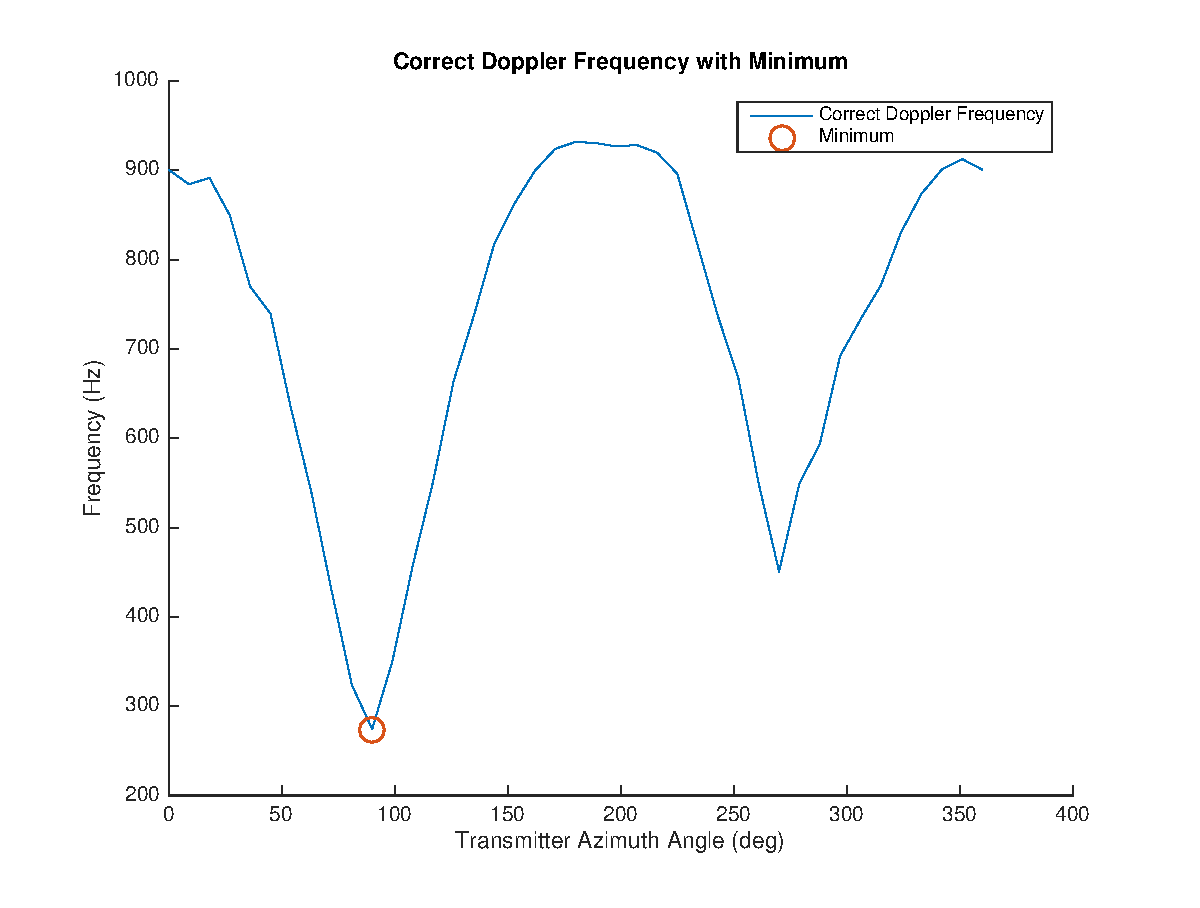
\includegraphics[width=10cm]{images/results/Correct_doppler_with_Minumum.eps}
		\caption{Correct Doppler Frequencies with Minimum vs Transmitter Azimuth Angle at an Elevation Angle of 45\textdegree}
		\label{fig:min_correct_fd}
	\end{center}
\end{figure}

In order to find the local minimum at 270\textdegree \space we need to use a different method.  We can do this through the peak detection function within MATLAB to locate both the 90\textdegree \space and 270\textdegree \space point. By taking the inverse of the correct Doppler and tuning the peak detection function with the maximum and minimum values to determine accurate prominence.

%matlab peak detection code with tuning params
\begin{lstlisting}
%peak detection with prominence calculation
min_peak_prominence = (1/(Max - Min))*.5;
[pk,lc] = findpeaks(1./correct_fd, 'NPeaks', 2, 'MinPeakProminence', min_peak_prominence);
\end{lstlisting}

%figure with peak detection plotted vs azimuth
\begin{figure}
	\begin{center}
		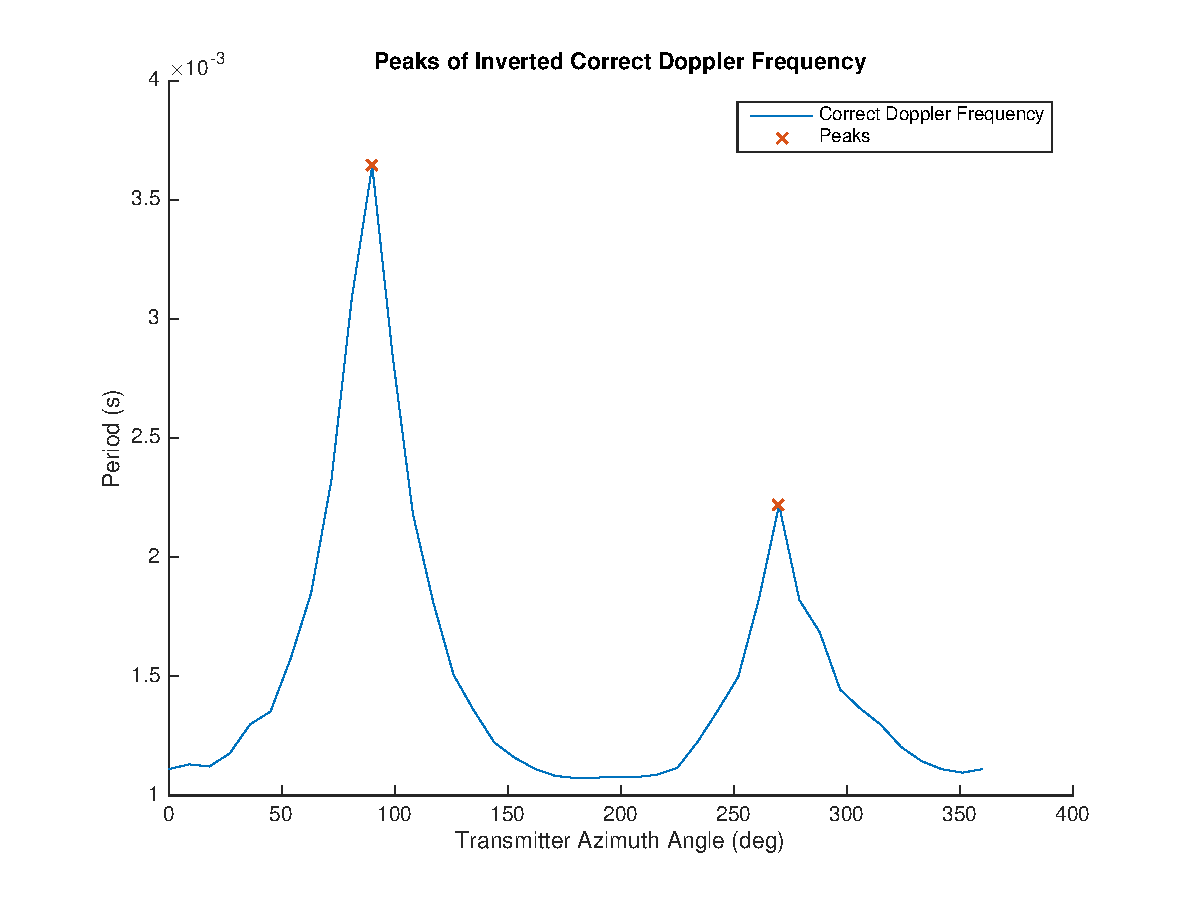
\includegraphics[width=10cm]{images/results/Correct_doppler_inverse_peaks.eps}
		\caption{Peaks of inverted Correct Doppler vs Transmitter Azimuth Angle at an Elevation Angle of 45\textdegree}
		\label{fig:peaks}
	\end{center}
\end{figure}

From Figure \ref{fig:peaks}  we see the two peaks denoted by the red x's, one at 90\textdegree \space and the other at  270\textdegree. Now we have a minimum value that should denote the 90\textdegree \space location and the two peak locations that denote the 90\textdegree \space and 270\textdegree \space locations. Since it is possible that the minimum could find the wrong peak for the 90\textdegree \space location we can compare the peak locations on the average power data, that was used to find the successive average during data collection, to determine which location is actually 90\textdegree.

%figure with power plot with 90 and 270 denoted
\begin{figure}
	\begin{center}
		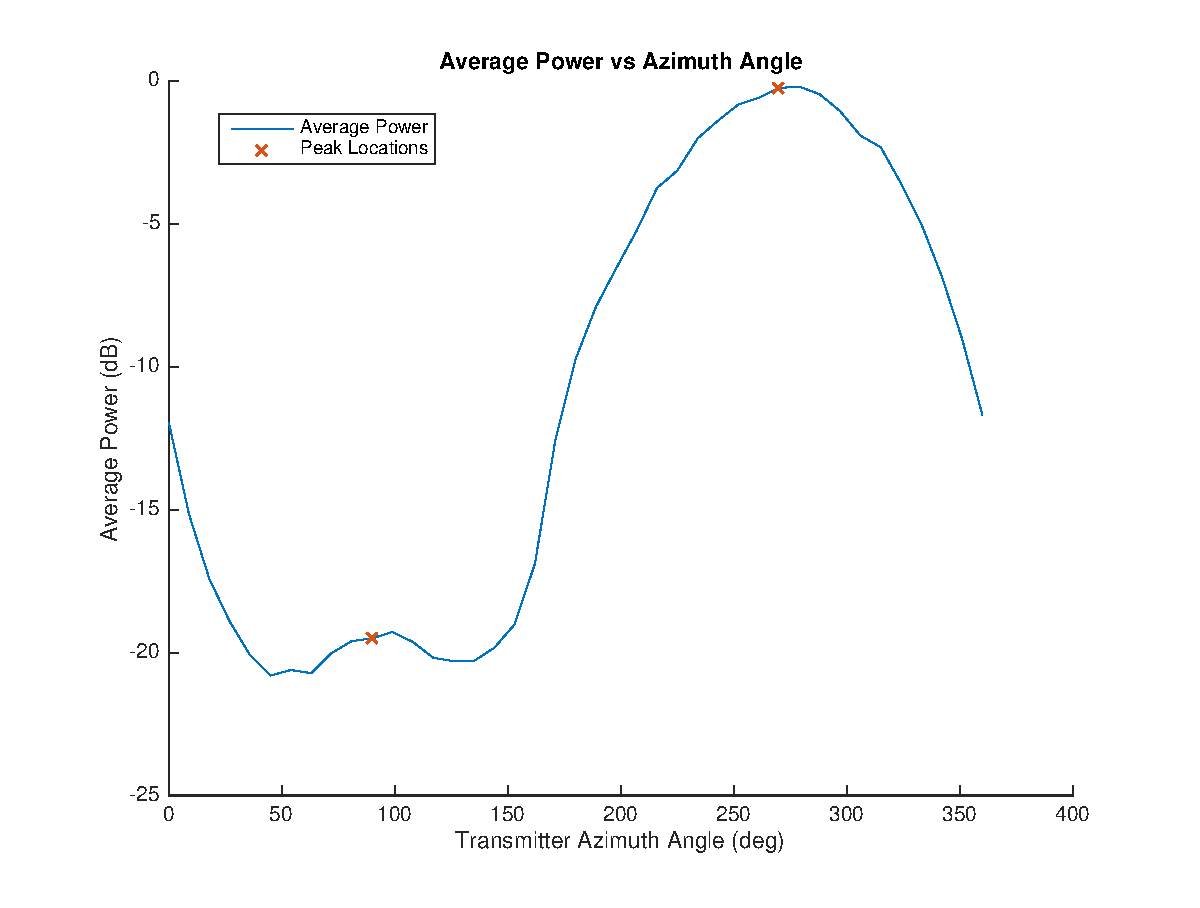
\includegraphics[width=10cm]{images/results/average_power_vs_Azimuth.eps}
		\caption{Average Power vs Transmitter Azimuth Angle at an Elevation Angle of 45\textdegree}
		\label{fig:ave_power}
	\end{center}
\end{figure}

Figure \ref{fig:ave_power}  shows the average power at each angle sample with the angles 90\textdegree \space and 270\textdegree \space denoted as red x's. From the plot we can see that the average power at 90\textdegree \space is much smaller than at 270\textdegree, so this inequality will be used to resolve ambiguity in the azimuth angle. 

From there the minimum method and the peak method can be compared to see if they agree on the 90\textdegree \space location. If this is not the case one will be chosen and the helicopter can fly in that direction. The resulting Doppler can then be measured, based on the physical movement of the helicopter or if the resulting profile, to confirm the correct 90\textdegree \space location. 

%azimuth error table
\begin{table}
\begin{center}
    \begin{tabular}{ | l | l | l | l |}
    \hline
    Altitude & Elevation Angle & Azimuth Error in (deg) & Percent Error \\ \hline
     200 & 76\textdegree & 0 & 0  \\ \hline
     200 & 45\textdegree & 0 & 0  \\ \hline 
     200 & 26.5\textdegree & 0 & 0  \\ \hline
     500 & 78.7\textdegree & 0 & 0  \\ \hline
     500 & 51.34\textdegree & 0 & 0  \\ \hline 
     500 & 35.5\textdegree & 0 & 0  \\ \hline
    \end{tabular}
     \caption{Azimuth Error and Azimuth Percent Error of Different Elevation Angles During Azimuth Estimation}
    \label{tab:az_error_and_percent}
\end{center}
\end{table}

From Table \ref{tab:az_error_and_percent} we can see that there is no error in the estimation of the 90\textdegree \space point over a variety of altitude and elevation angles that were tested. But because the algorithm could potentially pick the 270\textdegree \space we will analyze the difference in peak heights and the power difference to evaluate the estimation further.

\begin{table}
\begin{center}
    \begin{tabular}{ | l | l | p{3cm} | p{3cm} | p{3cm} |}
    \hline
    Altitude & Elevation Angle & Percent Peak Difference & Power Difference in dB & Peak Frequency Difference Hz\\ \hline
     200 & 76\textdegree & -16.8675\% & -14.0914  & 18.67 \\ \hline
     200 & 45\textdegree & -39.1124\% & -19.7476  &  176.267\\ \hline 
     200 & 26.5\textdegree & -69.7368\% & -13.3443 & 424.0 \\ \hline
     500 & 78.7\textdegree & -21.6667\% & -11.4508  & 17.33 \\ \hline
     500 & 51.34\textdegree & -38.1875\% & -22.4610  & 162.93 \\ \hline 
     500 & 35.5\textdegree & -53.4303\% & -18.6043  & 313.6 \\ \hline
    \end{tabular}
    \caption{Percent Peak, Power, and Frequency Difference of Different Elevation Angles During Azimuth Estimation}
    \label{tab:peaks_and_power}
\end{center}
\end{table}

From Table \ref{tab:peaks_and_power} we can see that at the larger elevation angles the peak percent difference are significant to determine which is correctly the 90\textdegree \space value. Although from the frequency difference, at the large elevation angles, it is possible to confuse the estimation by just taking the minimum frequency. Therefore other values need to play a role such as the received power.

%-----------------------------------------------------------------------------------------------------------------------------------------------------------------------

\section{Transmitter Elevation Angle Estimation} \label{sec:transmitter_elevation_angle_estimation}
%formulate the estimation equation and discuss ambiguity considerations
Using the information gathered from the azimuth estimation procedure, we can compute the elevation angle of the transmitter. In the process of gathering azimuth information, the maximum and minimum profiles follow a sinusoidal pattern that contains a maximum Doppler information at approximately 180\textdegree \space and 0\textdegree \space azimuth angles. Using that maximum value, along with the correct Doppler and the assumption that the maximum will occur near the tip of the rotor blade, we can approximate the respected reflection radii by:
%reflection radius aproximation equation
\begin{equation}
	R_{Estimate} = r_b \left(\frac{f_{DopplerCorrect}(\theta_{Az})}{Max(f_{DopplerCorrect})}\right)
	\label{eqn:r_estimate}
\end{equation}

where $R_{Estimate}$ is the estimated reflection radius at a particular azimuth, $r_b$ is the length of a single blade or radius of the rotor, and $f_{DopplerCorrect}$ is the correct Doppler frequency for each azimuth angle $\theta_{Az}$.

%figure of radius estimation 
\begin{figure}
	\begin{center}
		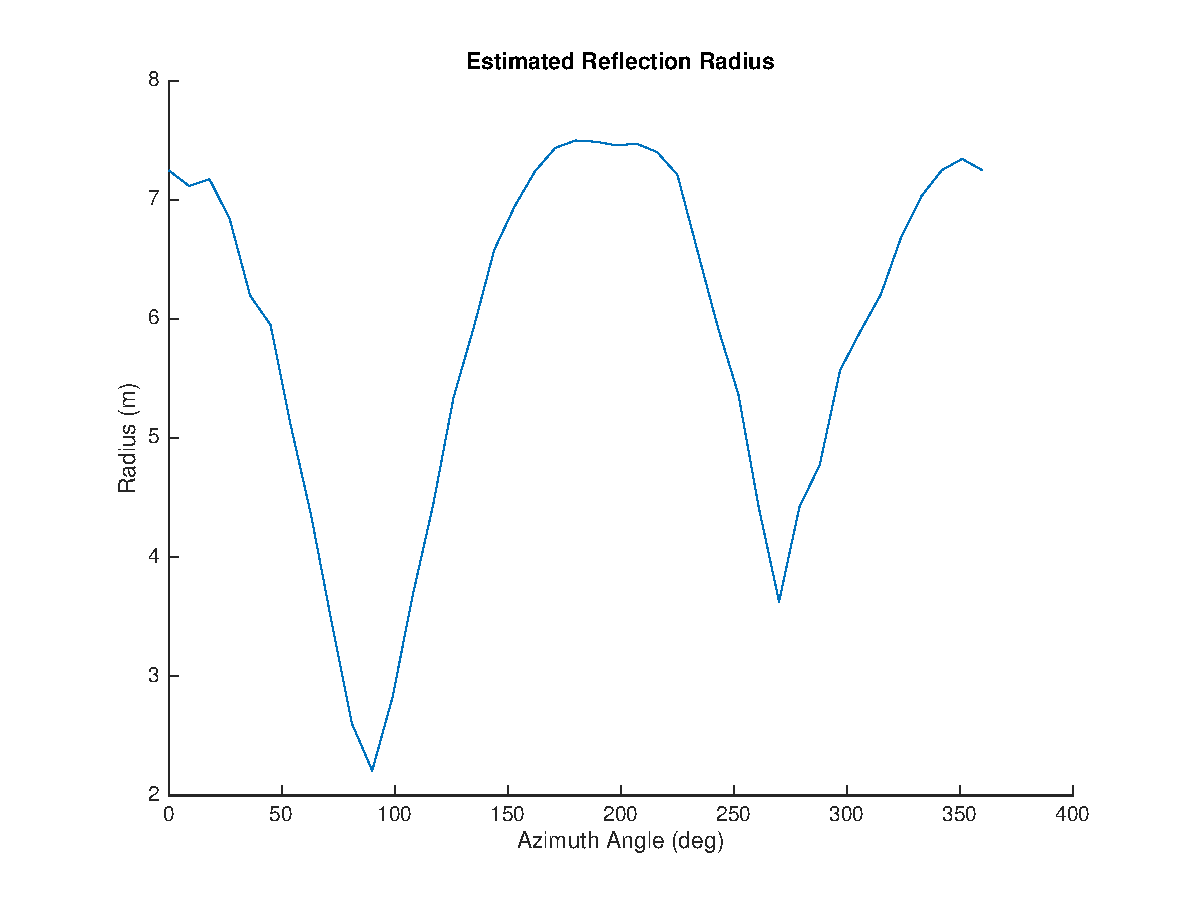
\includegraphics[width=10cm]{images/results/Estimated_reflection_radius_Azimuth_range.eps}
		\caption{Estimated Reflection Radius at an Elevation Angle of 45\textdegree}
		\label{fig:est_radius_azimuth_range}
	\end{center}
\end{figure}

Figure \ref{fig:est_radius_azimuth_range} shows the estimated reflection radius for each azimuth angle.

Now we find the maximum amount of Doppler that could be induced at that reflection radius location is:
%max doppler at radius location
\begin{equation}
	f_{Doppler_{R Estimate Max}} = 2\frac{v_r f_c}{c}
	\label{eqn:max_doppler}
\end{equation}

where $f_{Doppler_{R Estimate Max}}$ is the maximum amount of Doppler that could happen at that location if the signal was reflected parallel to the direction of motion. $f_c$ is the center frequency of the signal, $c$ is the speed of light and $v_r$ is the radial velocity based of the $\omega_r$ is:

%radial velocity
\begin{equation}
	v_r = \omega_r R_{Estimate}
	\label{eqn:v_radial}
\end{equation}

Then to find the elevation angle we look back at equation \ref{eq:theory_180_upper} swapping $MaxDopplerProfile$ with $f_{DopplerCorrect(\theta_{Az})}$ because this is now over the azimuth range and swap $f_{DopplerMax}$ for $f_{Doppler_{R Estimate Max}}$ because we need the maximum doppler for the current reflection estimate. We then solve for the elevation angle:

%Elevation angle
\begin{equation}
	\theta_{El} = acos\left(\frac{f_{DopplerCorrect(\theta_{Az})}}{f_{Doppler_{R Estimate Max}}}\right)
	\label{eqn:elevation_angle}
\end{equation}

where $\theta_{El}$ is the elevation angle of the transmitter. If the elevation angle is all the information needed equation \ref{eqn:elevation_angle} distills down to:

%Elevation angle
\begin{equation}
	\theta_{El} = acos\left(\frac{Max(f_{DopplerCorrect})}{f_{DopplerMax}}\right)
	\label{eqn:elevation_angle_only}
\end{equation}

where $f_{DopplerMax}$ is defined in equation \ref{eqn:fd_max}.

%figure of elevation angle 
\begin{figure}
	\begin{center}
		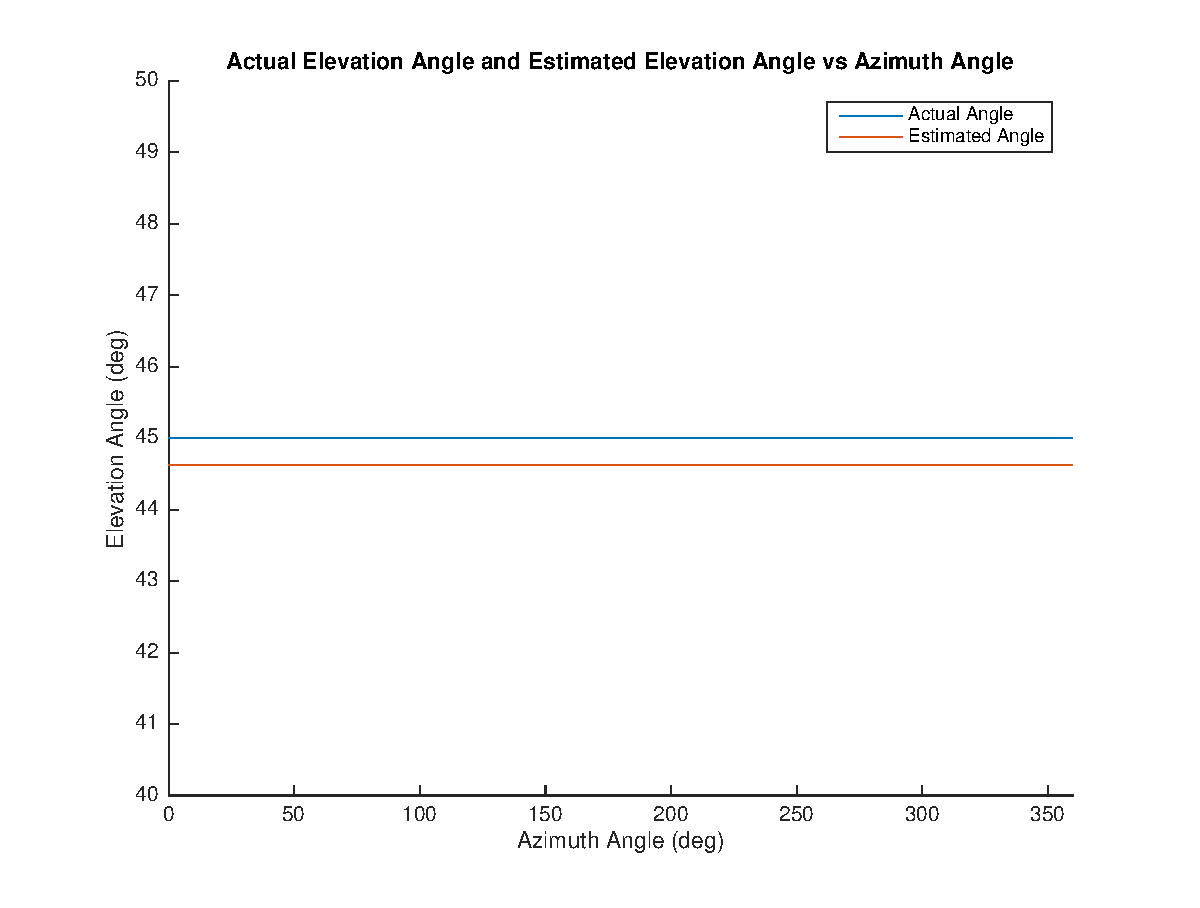
\includegraphics[width=10cm]{images/results/Elevation_angle_comparason_Azimuth_range.eps}
		\caption{Actual Elevation Angle and Estimated Elevation Angle vs Azimuth Angle}
		\label{fig:elevation_comparason_azimuth_range}
	\end{center}
\end{figure}

Figure \ref{fig:elevation_comparason_azimuth_range} shows the estimation of the elevation angle $\theta_{El}$ with respect to the azimuth angle. What it shows is that the elevation angle remains constant with respect to azimuth angle. Which means that the estimation in the reflection radius is correctly compensating for the azimuth angle. The percent error off the actual elevation angle is shown in Figure \ref{fig:percent_error_elevation_azimuth_range} which is very small but consistent over the azimuth range.

%figure of percent error
\begin{figure}
	\begin{center}
		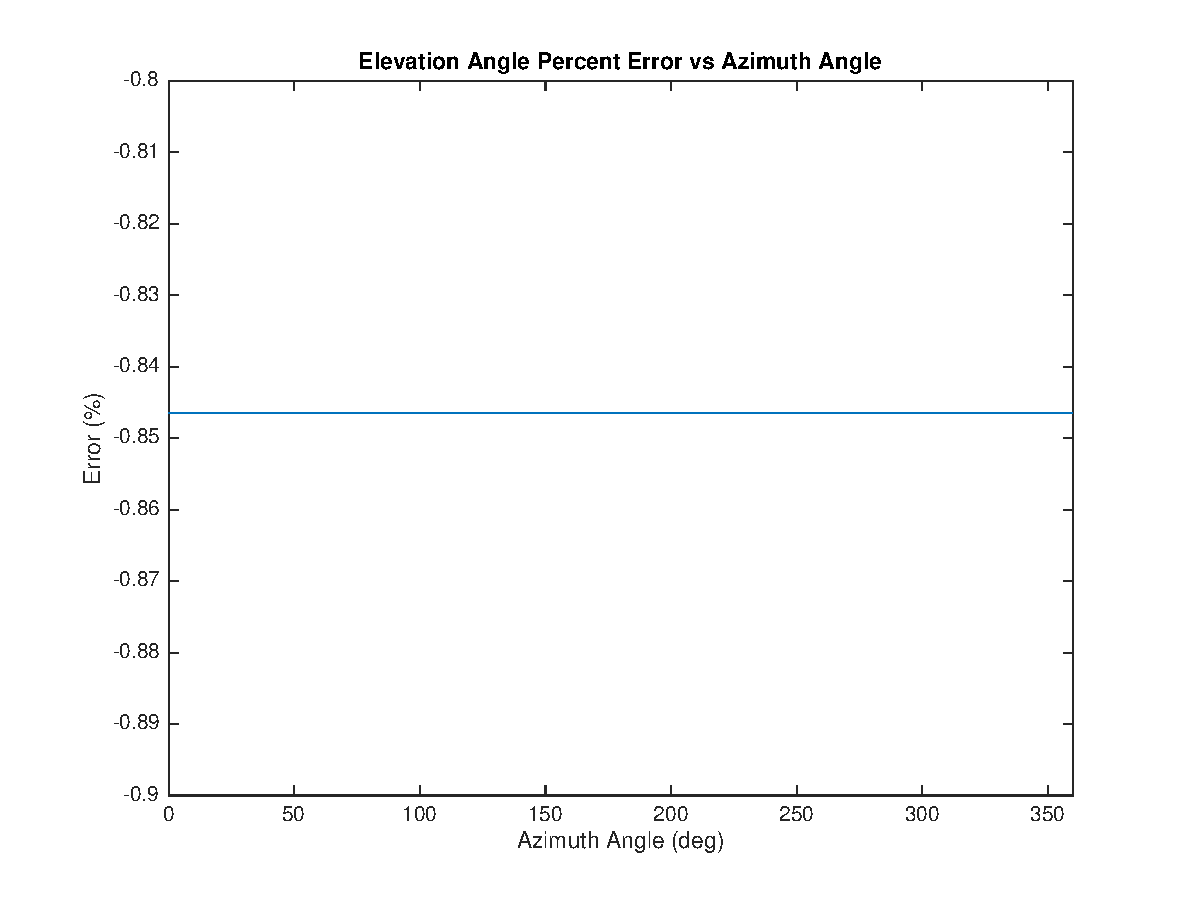
\includegraphics[width=10cm]{images/results/Elevation_angle_percent_error_Azimuth_range.eps}
		\caption{Elevation Angle Percent Error vsTransmitter Azimuth Angle}
		\label{fig:percent_error_elevation_azimuth_range}
	\end{center}
\end{figure}

% Elevation error table
\begin{table}
\begin{center}
    \begin{tabular}{ | l | l | l | l |}
    \hline
    Altitude & Elevation Angle & Average Elevation Error in (deg) & Average Percent Error \\ \hline
     200 & 76\textdegree & -0.4632\textdegree & -0.6097\%  \\ \hline
     200 & 45\textdegree & -0.3809\textdegree & -0.8464\%  \\ \hline 
     200 & 26.5\textdegree & -0.4072\textdegree & -1.5329\%  \\ \hline
     500 & 78.7\textdegree & 0.0914\textdegree & 0.1162\% \\ \hline
     500 & 51.34\textdegree & -0.6236\textdegree & -1.2146\%  \\ \hline 
     500 & 35.5\textdegree & -0.6803\textdegree & -1.9143\%  \\ \hline
    \end{tabular}
    \caption{Average Elevation Error and Average Elevation Percent Error of Different Elevation Angles During Azimuth Estimation}
    \label{tab:elevation_error_percent}
\end{center}
\end{table}

From Table \ref{tab:elevation_error_percent} we can see elevation estimation error is extremely small for the given elevation angles. There is a trend that is evident in the data that as the elevation angle decreases the amount of error is increasing.

%-----------------------------------------------------
% range limitations of this aproximation
%-----------------------------------------------------

The error in elevation is caused by a limitation on the estimation. Where the Doppler shift is limited by the maximum amount Doppler that the blade rotation can produce shown in equation \ref{eqn:v_radial} by replacing $v_r$ with $v_rMax$ which is:

%radial velocity
\begin{equation}
	v_{rMax} = \omega_r r_b
	\label{eqn:v_radial_max}
\end{equation}

then using $v_{rMax}$ to find the maximum available Doppler:

%maximum available doppler
\begin{equation}
	f_{DopplerMax} = 2\frac{v_{rMax} f_c}{c}
	\label{eqn:fd_max}
\end{equation}

This limitation is shown by varying the elevation angle at the azimuth angle that provides the maximum Doppler shift, which is 180\textdegree. The maximum and minimum profile data is shown in Figure \ref{fig:envelope_180deg}

%figure of 180 deg elevation sweep of envelope
\begin{figure}
	\begin{center}
		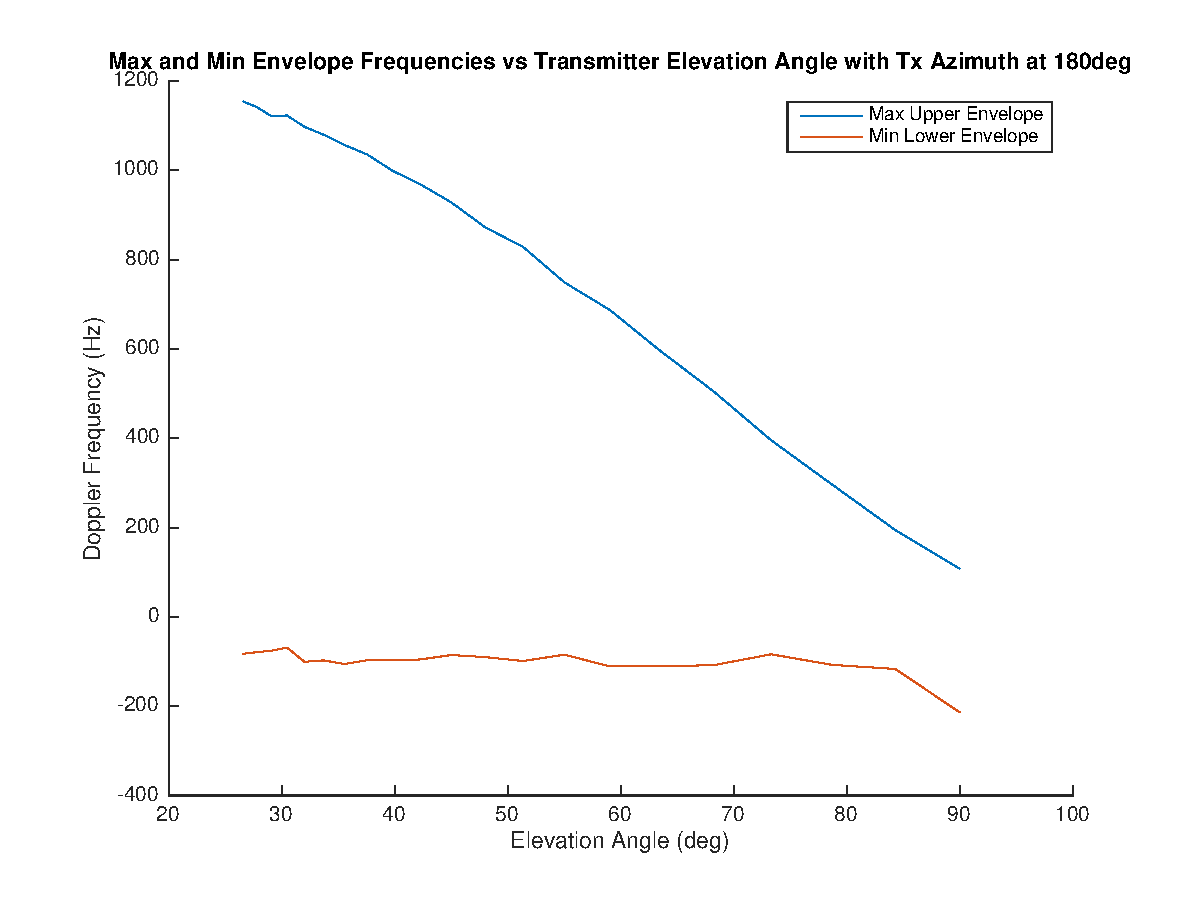
\includegraphics[width=10cm]{images/simulation/elevation_angle_max_doppler_180deg.eps}
		\caption{Max and Min Doppler Profile Frequencies vs Elevation Angle with Transmitter Azimuth Angle of 180\textdegree}
		\label{fig:envelope_180deg}
	\end{center}
\end{figure}

%figure of comparing actual to estimated
\begin{figure}
	\begin{center}
		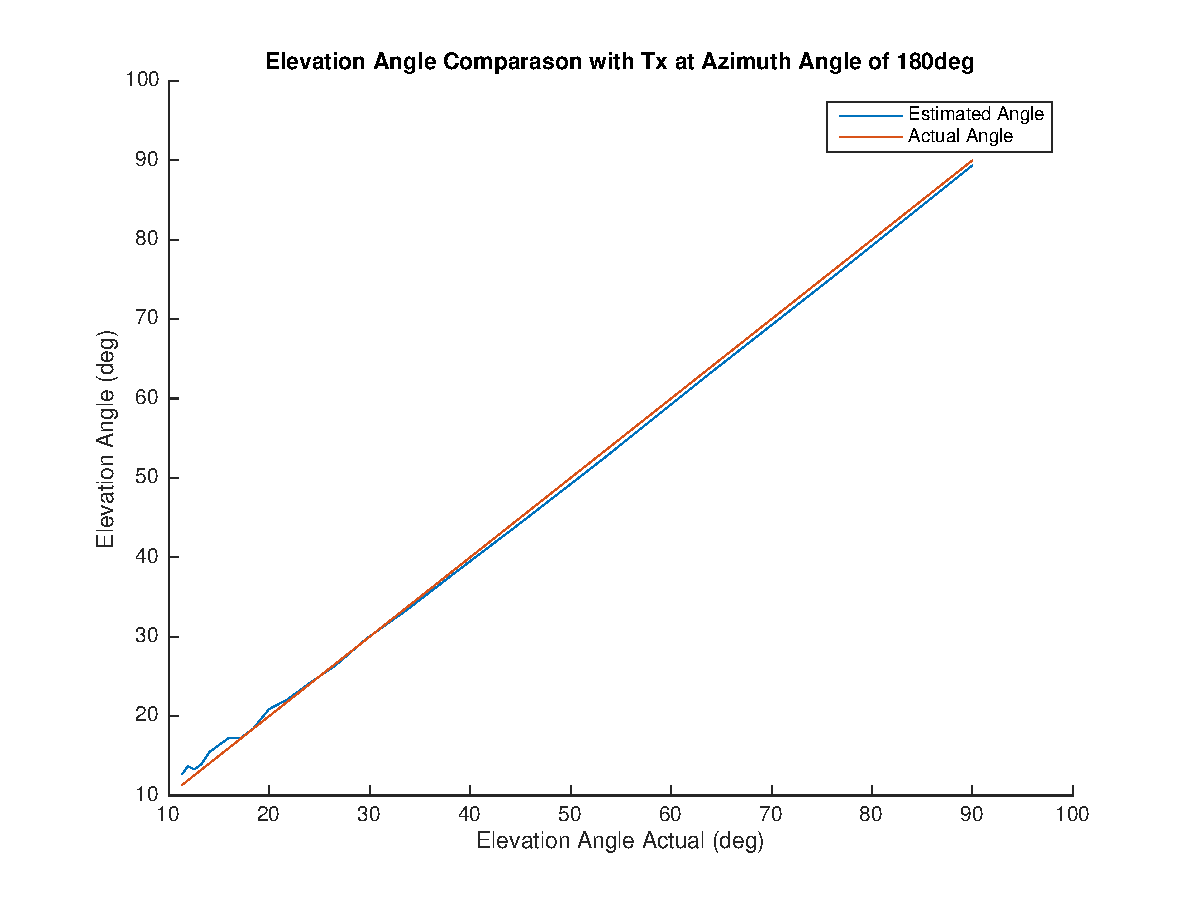
\includegraphics[width=10cm]{images/results/Elevation_angle_comparason_180deg_Azimuth.eps}
		\caption{Elevation Estimate and Actual Angle with Transmitter Azimuth Angle of 180\textdegree}
		\label{fig:angle_comparason_180deg}
	\end{center}
\end{figure}

Using the estimation method described above, Figure \ref{fig:angle_comparason_180deg} shows the elevation angle estimated versus the actual angle. The estimation method is accurate till elevation angles of 18\textdegree \space or 20\textdegree, where it becomes noisy. This is due to the inability of the profile estimation to resolve the correct maximum Doppler for that range. By going back to Figure \ref{fig:tx_range_elevation_rel} we can see that as the transmitter moves farther and farther away the elevation angle is still decreasing but at a much smaller and smaller rate. So the difference between elevation angles closer to zero are more difficult to resolve. 

%figure percent error of increasing error and variability
\begin{figure}
	\begin{center}
		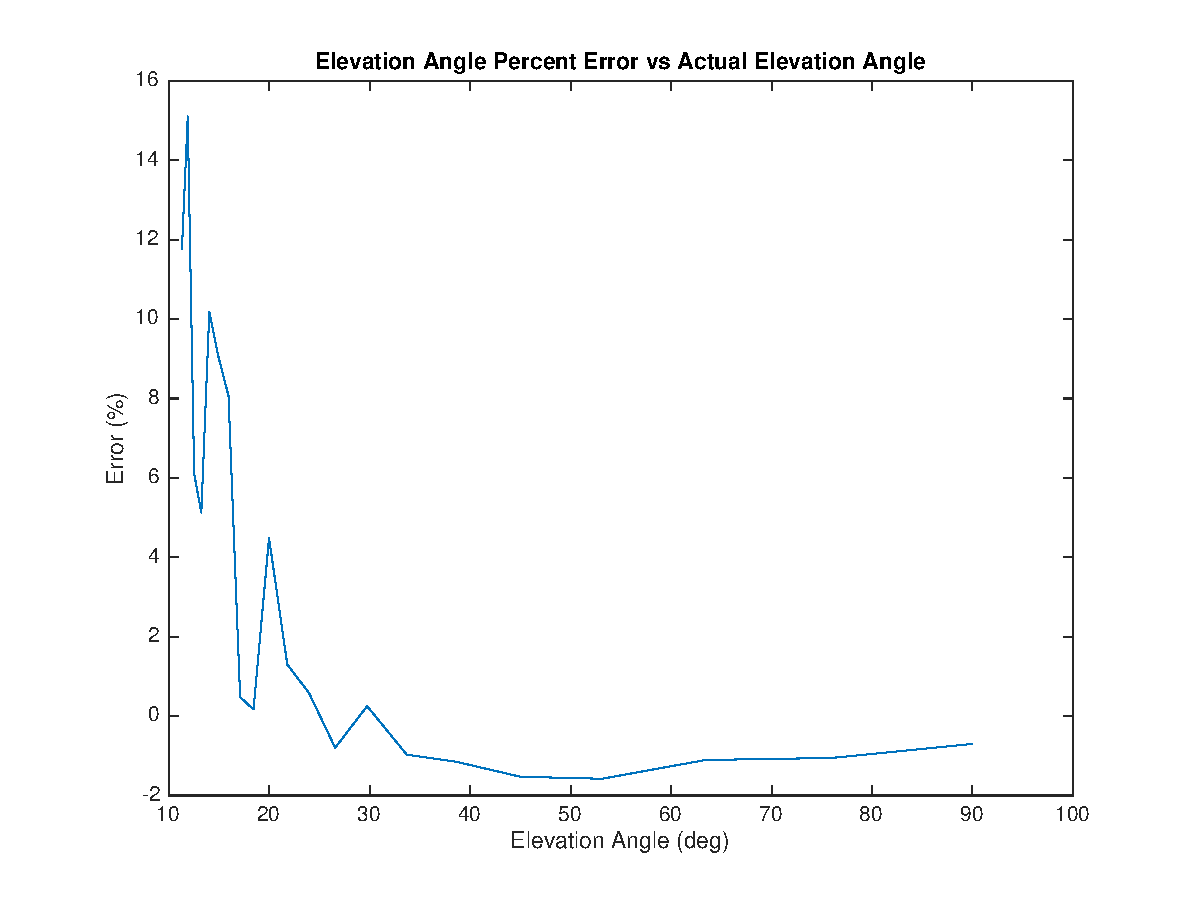
\includegraphics[width=10cm]{images/results/Elevation_angle_percent_error_180deg_Azimuth.eps}
		\caption{Elevation Angle Percent Error with Transmitter Azimuth Angle of 180\textdegree}
		\label{fig:percent_error_elevation_180deg}
	\end{center}
\end{figure}

Figure \ref{fig:percent_error_elevation_180deg} shows the percent error with respect to the elevation angle. The estimation starts to become unusable around 18\textdegree \space or 20\textdegree \space where the percent error starts to shoot past acceptable ranges.

%------------------------------
%pitch considerations
%------------------------------

If we now consider a pitched blade the above method for estimating azimuth and elevation becomes inaccurate due to the increased Doppler between 90\textdegree \space and 270\textdegree \space and the decreased Doppler on the other side. To correct this error we need to correct both the difference calculation and the correct Doppler data accordingly. The uncorrected data is shown in Figure \ref{fig:diff_pitch_noCorrection} and \ref{fig:dop_pitch_noCorrection} with percent azimuth error of 20\% and percent elevation error of 35\%.

\begin{figure}
	\begin{center}
		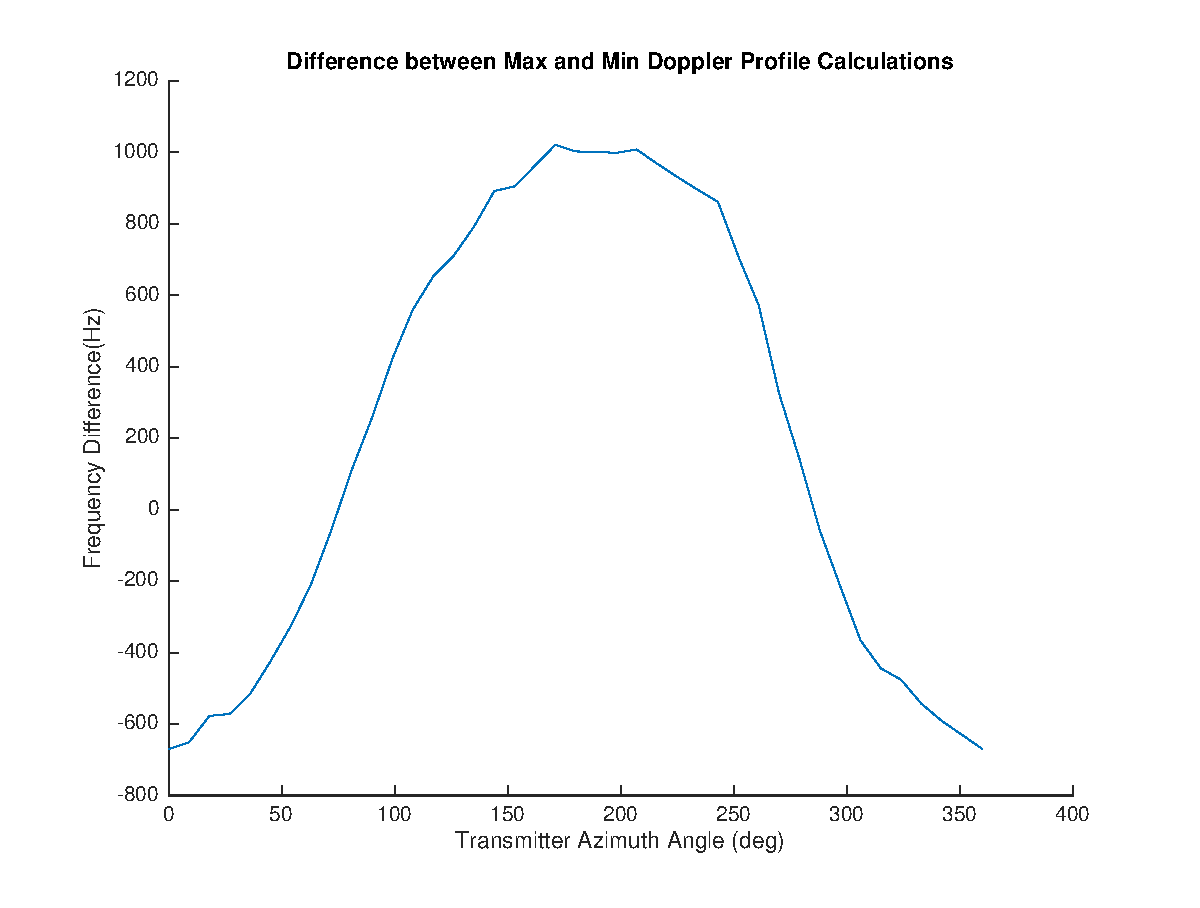
\includegraphics[width=10cm]{images/results/difference_pitch_noCorrection.eps}
		\caption{Uncorrected Doppler Profile Difference vs. Transmitter Azimuth and Elevation angle of 45\textdegree with Blade pitch of 7.5\textdegree}
		\label{fig:diff_pitch_noCorrection}
	\end{center}
\end{figure}

\begin{figure}
	\begin{center}
		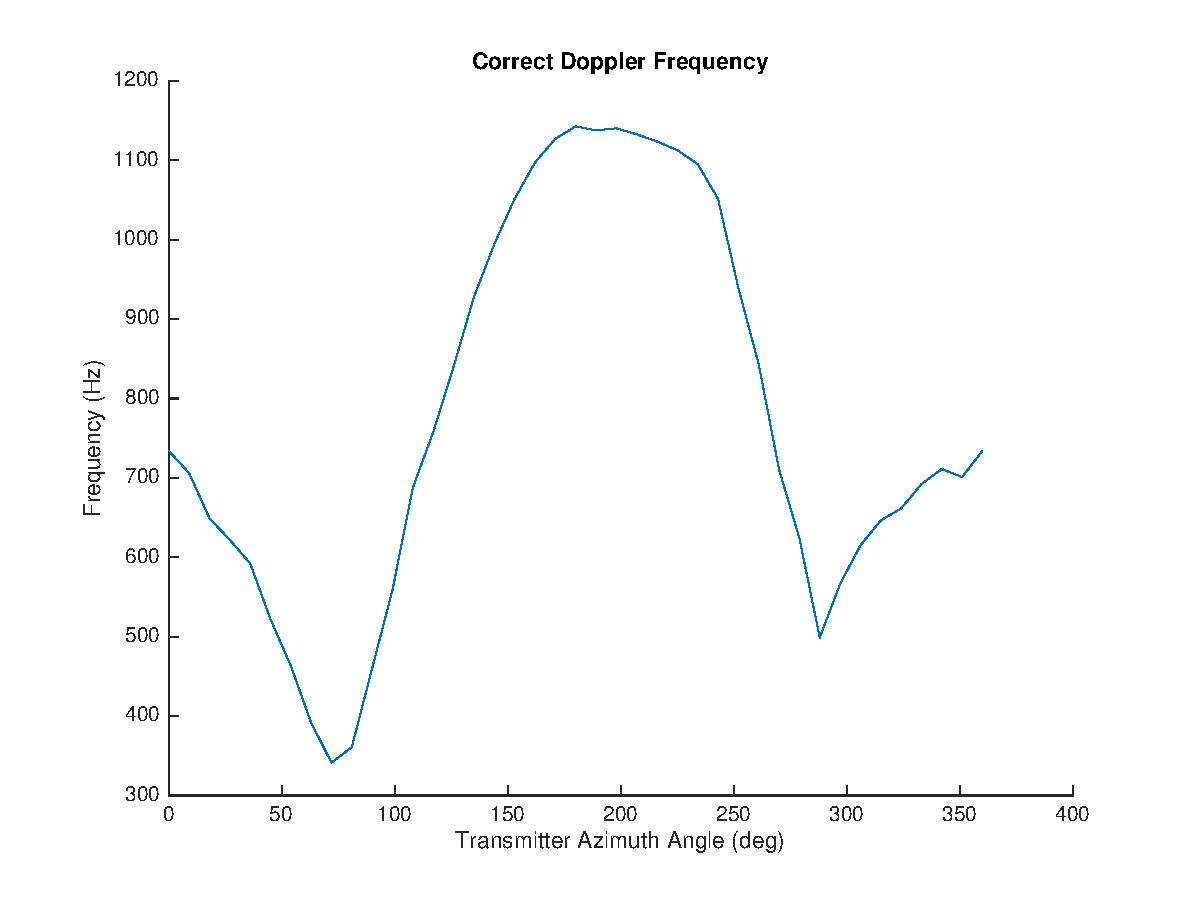
\includegraphics[width=10cm]{images/results/correct_dop_pitch_noCorrection.eps}
		\caption{Uncorrected Pitch Doppler Profile vs. Transmitter Azimuth and Elevation angle of 45\textdegree with Blade pitch of 7.5\textdegree}
		\label{fig:dop_pitch_noCorrection}
	\end{center}
\end{figure}

Comparing the Doppler profile difference of no pitch and pitched blade, in Figures \ref{fig:azimuth_estimation_difference} and \ref{fig:diff_pitch_noCorrection} respectively, we can see that the difference calculation of the pitch is a shifted up version of the one with no pitch. Therefore we can first correct this by re-centering the pitch difference: 

\begin{equation}
	A_{shift} = \frac{Max(Max Doppler Profile) - |Min(Min Doppler Profile)|}{2}
	\label{eqn:pitch_shift}
\end{equation}

where $A_{shift}$ is the amount that the difference calculation will be shifted:

\begin{equation}
	ProfileDifference = ProfileDifference - A_{shift}
	\label{eqn:diff_shift}
\end{equation}

Then $f_{DopplerCorrect}$ is recalculated and then adjusted to the correct frequencies:

%fix correct doppler for pitch
\begin{equation}
	f_{DopplerCorrect} = f_{DopplerCorrect} + A_{shift}cos\left(\theta_{Az}\right)
	\label{eqn:fd_pitch_correct}
\end{equation}

Since $\theta_{Az}$ is unknown during the calculation of equation \ref{eqn:fd_pitch_correct} the correct starting phase can be determined by matching it to the $ProfileDifference$ and that the cosine should be one period in length. These corrections result in the percent azimuth error of 0\% and 7\% elevation angle error. The elevation angle percent error is within a useable range but could be decreased with further tuning to the preliminary pitch adjustment algorithm. When the pitch corrections are applied to a transmitter elevation angle of 26.56\textdegree \space the correction achieves better performance than the unpitched calculation with percent azimuth error of 0\% and percent elevation error of 0.114\%. This is still a preliminary correction method that requires more in depth analysis but from the initial results shows merit. The increased accuracy as the elevation angle decreases relates back to Figure \ref{fig:pitch_tx_elevation_angle} where as the elevation angle decreases the effect of pitch on the signal converges back to the unpitched results.



